% Options for packages loaded elsewhere
\PassOptionsToPackage{unicode}{hyperref}
\PassOptionsToPackage{hyphens}{url}
%
\documentclass[
]{article}
\usepackage{lmodern}
\usepackage{amssymb,amsmath}
\usepackage{ifxetex,ifluatex}
\ifnum 0\ifxetex 1\fi\ifluatex 1\fi=0 % if pdftex
  \usepackage[T1]{fontenc}
  \usepackage[utf8]{inputenc}
  \usepackage{textcomp} % provide euro and other symbols
\else % if luatex or xetex
  \usepackage{unicode-math}
  \defaultfontfeatures{Scale=MatchLowercase}
  \defaultfontfeatures[\rmfamily]{Ligatures=TeX,Scale=1}
\fi
% Use upquote if available, for straight quotes in verbatim environments
\IfFileExists{upquote.sty}{\usepackage{upquote}}{}
\IfFileExists{microtype.sty}{% use microtype if available
  \usepackage[]{microtype}
  \UseMicrotypeSet[protrusion]{basicmath} % disable protrusion for tt fonts
}{}
\makeatletter
\@ifundefined{KOMAClassName}{% if non-KOMA class
  \IfFileExists{parskip.sty}{%
    \usepackage{parskip}
  }{% else
    \setlength{\parindent}{0pt}
    \setlength{\parskip}{6pt plus 2pt minus 1pt}}
}{% if KOMA class
  \KOMAoptions{parskip=half}}
\makeatother
\usepackage{xcolor}
\IfFileExists{xurl.sty}{\usepackage{xurl}}{} % add URL line breaks if available
\IfFileExists{bookmark.sty}{\usepackage{bookmark}}{\usepackage{hyperref}}
\hypersetup{
  pdftitle={Moberg Analytics HDF5 Documentation},
  pdfauthor={Author: Zack Goldblum - Moberg Analytics},
  hidelinks,
  pdfcreator={LaTeX via pandoc}}
\urlstyle{same} % disable monospaced font for URLs
\usepackage[margin=1in]{geometry}
\usepackage{color}
\usepackage{fancyvrb}
\newcommand{\VerbBar}{|}
\newcommand{\VERB}{\Verb[commandchars=\\\{\}]}
\DefineVerbatimEnvironment{Highlighting}{Verbatim}{commandchars=\\\{\}}
% Add ',fontsize=\small' for more characters per line
\usepackage{framed}
\definecolor{shadecolor}{RGB}{248,248,248}
\newenvironment{Shaded}{\begin{snugshade}}{\end{snugshade}}
\newcommand{\AlertTok}[1]{\textcolor[rgb]{0.94,0.16,0.16}{#1}}
\newcommand{\AnnotationTok}[1]{\textcolor[rgb]{0.56,0.35,0.01}{\textbf{\textit{#1}}}}
\newcommand{\AttributeTok}[1]{\textcolor[rgb]{0.77,0.63,0.00}{#1}}
\newcommand{\BaseNTok}[1]{\textcolor[rgb]{0.00,0.00,0.81}{#1}}
\newcommand{\BuiltInTok}[1]{#1}
\newcommand{\CharTok}[1]{\textcolor[rgb]{0.31,0.60,0.02}{#1}}
\newcommand{\CommentTok}[1]{\textcolor[rgb]{0.56,0.35,0.01}{\textit{#1}}}
\newcommand{\CommentVarTok}[1]{\textcolor[rgb]{0.56,0.35,0.01}{\textbf{\textit{#1}}}}
\newcommand{\ConstantTok}[1]{\textcolor[rgb]{0.00,0.00,0.00}{#1}}
\newcommand{\ControlFlowTok}[1]{\textcolor[rgb]{0.13,0.29,0.53}{\textbf{#1}}}
\newcommand{\DataTypeTok}[1]{\textcolor[rgb]{0.13,0.29,0.53}{#1}}
\newcommand{\DecValTok}[1]{\textcolor[rgb]{0.00,0.00,0.81}{#1}}
\newcommand{\DocumentationTok}[1]{\textcolor[rgb]{0.56,0.35,0.01}{\textbf{\textit{#1}}}}
\newcommand{\ErrorTok}[1]{\textcolor[rgb]{0.64,0.00,0.00}{\textbf{#1}}}
\newcommand{\ExtensionTok}[1]{#1}
\newcommand{\FloatTok}[1]{\textcolor[rgb]{0.00,0.00,0.81}{#1}}
\newcommand{\FunctionTok}[1]{\textcolor[rgb]{0.00,0.00,0.00}{#1}}
\newcommand{\ImportTok}[1]{#1}
\newcommand{\InformationTok}[1]{\textcolor[rgb]{0.56,0.35,0.01}{\textbf{\textit{#1}}}}
\newcommand{\KeywordTok}[1]{\textcolor[rgb]{0.13,0.29,0.53}{\textbf{#1}}}
\newcommand{\NormalTok}[1]{#1}
\newcommand{\OperatorTok}[1]{\textcolor[rgb]{0.81,0.36,0.00}{\textbf{#1}}}
\newcommand{\OtherTok}[1]{\textcolor[rgb]{0.56,0.35,0.01}{#1}}
\newcommand{\PreprocessorTok}[1]{\textcolor[rgb]{0.56,0.35,0.01}{\textit{#1}}}
\newcommand{\RegionMarkerTok}[1]{#1}
\newcommand{\SpecialCharTok}[1]{\textcolor[rgb]{0.00,0.00,0.00}{#1}}
\newcommand{\SpecialStringTok}[1]{\textcolor[rgb]{0.31,0.60,0.02}{#1}}
\newcommand{\StringTok}[1]{\textcolor[rgb]{0.31,0.60,0.02}{#1}}
\newcommand{\VariableTok}[1]{\textcolor[rgb]{0.00,0.00,0.00}{#1}}
\newcommand{\VerbatimStringTok}[1]{\textcolor[rgb]{0.31,0.60,0.02}{#1}}
\newcommand{\WarningTok}[1]{\textcolor[rgb]{0.56,0.35,0.01}{\textbf{\textit{#1}}}}
\usepackage{longtable,booktabs}
% Correct order of tables after \paragraph or \subparagraph
\usepackage{etoolbox}
\makeatletter
\patchcmd\longtable{\par}{\if@noskipsec\mbox{}\fi\par}{}{}
\makeatother
% Allow footnotes in longtable head/foot
\IfFileExists{footnotehyper.sty}{\usepackage{footnotehyper}}{\usepackage{footnote}}
\makesavenoteenv{longtable}
\usepackage{graphicx,grffile}
\makeatletter
\def\maxwidth{\ifdim\Gin@nat@width>\linewidth\linewidth\else\Gin@nat@width\fi}
\def\maxheight{\ifdim\Gin@nat@height>\textheight\textheight\else\Gin@nat@height\fi}
\makeatother
% Scale images if necessary, so that they will not overflow the page
% margins by default, and it is still possible to overwrite the defaults
% using explicit options in \includegraphics[width, height, ...]{}
\setkeys{Gin}{width=\maxwidth,height=\maxheight,keepaspectratio}
% Set default figure placement to htbp
\makeatletter
\def\fps@figure{htbp}
\makeatother
\setlength{\emergencystretch}{3em} % prevent overfull lines
\providecommand{\tightlist}{%
  \setlength{\itemsep}{0pt}\setlength{\parskip}{0pt}}
\setcounter{secnumdepth}{5}
\usepackage[]{natbib}
\bibliographystyle{plainnat}

\title{Moberg Analytics HDF5 Documentation}
\author{Author: Zack Goldblum - Moberg Analytics}
\date{}

\begin{document}
\maketitle

{
\setcounter{tocdepth}{2}
\tableofcontents
}
\hypertarget{overview}{%
\section{Overview}\label{overview}}

This documentation details how to use the functions available in the \href{https://test.pypi.org/project/Moberg-Analytics-HDF5/}{Moberg-Analytics-HDF5 package}. The Moberg-Analytics-HDF5 package provides user-friendly functions organized into classes for reading HDF5 file content and components into Python. It is built on top of the \href{https://www.h5py.org/}{h5py package} which interfaces directly with the HDF5 file.

The three \textbf{HDF5Content}, \textbf{HDF5Components}, and \textbf{HDF5Helper} sections in the left-hand navigation bar correspond to the three classes within the hdf5\_tools module:

\begin{itemize}
\item
  \textbf{HDF5Content} contains functions that organize the contents of the HDF5 file into lists and dictionaries.
\item
  \textbf{HDF5Components} contains functions that return various components of the HDF5 file to the user including groups, datasets, Pandas/NumPy matrices of dataset values, metadata, and structured dictionaries.
\item
  \textbf{HDF5Helper} contains functions for argument, group, dataset, and duplicate checks as well as other methods that add functionality to HDF5Content and HDF5Components.
\end{itemize}

Each class section is further divided into \textbf{Group Functions}, \textbf{Dataset Functions}, and \textbf{Misc. Functions} sections that contain the relevant functions for working with groups, datasets, and other aspects of the HDF5 file. Every function has a description that details what it does, the parameters it accepts (if any), and what it returns. There are also code examples that demonstrate how the function is called and show what it returns. All of the code examples use the example.h5 HDF5 file, the structure of which is shown below.

\hypertarget{example-hdf5-file-structure}{%
\subsection{Example HDF5 File Structure}\label{example-hdf5-file-structure}}

\begin{figure}
\centering
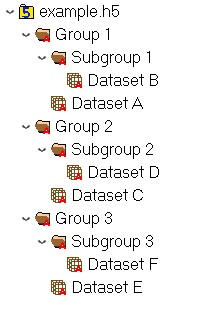
\includegraphics{resources/example_file_structure.jpg}
\caption{example.h5 in HDFView 3.1.1}
\end{figure}

\hypertarget{revision-history}{%
\subsection{Revision History}\label{revision-history}}

Date

Revision Number

Description

01/08/2021

1.0

Documentation created.

03/05/2021

2.0

Updated for package release.

\hypertarget{hdf5content}{%
\section{HDF5Content}\label{hdf5content}}

\emph{DESCRIPTION:}

This class contains functions that organize the contents of the HDF5 file into lists and dictionaries.

\emph{PARAMETERS:}

\begin{itemize}
\item
  \textbf{hdf5\_filepath}: HDF5 file path

  path to the user-selected HDF5 file
\end{itemize}

\emph{ATTRIBUTES:}

\begin{itemize}
\item
  \textbf{hdf5file}: HDF5 file

  user-selected HDF5 file
\item
  \textbf{all\_group\_names\_dict}: dict

  dictionary of every group and its associated info. Group names are keys.
\item
  \textbf{all\_dataset\_names\_dict}: dict

  dictionary of all datasets and their associated info. Datasetset names are keys.
\item
  \textbf{all\_dataset\_paths\_dict}: dict

  dictionary of all datasets and their associated info. Datasetset paths are keys.
\end{itemize}

\emph{EXAMPLE:}

\begin{Shaded}
\begin{Highlighting}[]
\CommentTok{# Path to the HDF5 file in your system directory}
\NormalTok{hdf5_filepath }\OperatorTok{=} \VerbatimStringTok{r"resources\textbackslash{}example.h5"}

\CommentTok{# Instantiate the HDF5Content class}
\NormalTok{hdf5_content }\OperatorTok{=}\NormalTok{ hdf5_tools.HDF5Content(hdf5_filepath}\OperatorTok{=}\NormalTok{hdf5_filepath)}
\end{Highlighting}
\end{Shaded}

\hypertarget{group-functions}{%
\subsection{Group Functions}\label{group-functions}}

\hypertarget{get_all_group_paths}{%
\subsubsection{get\_all\_group\_paths}\label{get_all_group_paths}}

\textbf{get\_all\_group\_paths()}

\emph{DESCRIPTION:}

Returns a list of all group paths in the HDF5 file (including the Root group and subgroups).

\emph{PARAMETERS:}

none

\emph{RETURNS:}

\begin{itemize}
\item
  \textbf{all\_group\_paths\_list}: list

  list of all group paths
\end{itemize}

\emph{EXAMPLE:}

\begin{Shaded}
\begin{Highlighting}[]
\NormalTok{all_group_paths_list }\OperatorTok{=}\NormalTok{ hdf5_content.get_all_group_paths()}
\end{Highlighting}
\end{Shaded}

\begin{verbatim}
## ['/',
##  'Group 1',
##  'Group 1/Subgroup 1',
##  'Group 2',
##  'Group 2/Subgroup 2',
##  'Group 3',
##  'Group 3/Subgroup 3']
\end{verbatim}

\hypertarget{get_all_group_objs}{%
\subsubsection{get\_all\_group\_objs}\label{get_all_group_objs}}

\textbf{get\_all\_group\_objs()}

\emph{DESCRIPTION:}

Returns a list of all group class objects in the HDF5 file (including the Root group and subgroups).

\emph{PARAMETERS:}

none

\emph{RETURNS:}

\begin{itemize}
\item
  \textbf{all\_group\_objs\_list}: list

  list of all HDF5 group class objects
\end{itemize}

\emph{EXAMPLE:}

\begin{Shaded}
\begin{Highlighting}[]
\NormalTok{all_group_objs_list }\OperatorTok{=}\NormalTok{ hdf5_content.get_all_group_objs()}
\end{Highlighting}
\end{Shaded}

\begin{verbatim}
## [<HDF5 group "/" (3 members)>,
##  <HDF5 group "/Group 1" (2 members)>,
##  <HDF5 group "/Group 1/Subgroup 1" (1 members)>,
##  <HDF5 group "/Group 2" (2 members)>,
##  <HDF5 group "/Group 2/Subgroup 2" (1 members)>,
##  <HDF5 group "/Group 3" (2 members)>,
##  <HDF5 group "/Group 3/Subgroup 3" (1 members)>]
\end{verbatim}

\hypertarget{get_all_group_names}{%
\subsubsection{get\_all\_group\_names}\label{get_all_group_names}}

\textbf{get\_all\_group\_names()}

\emph{DESCRIPTION:}

Returns a list of all group names in the HDF5 file (including the Root group and subgroups).

\emph{PARAMETERS:}

none

\emph{RETURNS:}

\begin{itemize}
\item
  \textbf{all\_group\_names\_list}: list

  list of all group names
\end{itemize}

\emph{EXAMPLE:}

\begin{Shaded}
\begin{Highlighting}[]
\NormalTok{all_group_names_list }\OperatorTok{=}\NormalTok{ hdf5_content.get_all_group_names()}
\end{Highlighting}
\end{Shaded}

\begin{verbatim}
## ['/', 'Group 1', 'Subgroup 1', 'Group 2', 'Subgroup 2', 'Group 3', 'Subgroup 3']
\end{verbatim}

\hypertarget{get_all_group_names_dict}{%
\subsubsection{get\_all\_group\_names\_dict}\label{get_all_group_names_dict}}

\textbf{get\_all\_group\_names\_dict()}

\emph{DESCRIPTION:}

Returns a dictionary of all group names (including the Root group and subgroups) and their associated info from the HDF5 file.

\emph{PARAMETERS:}

none

\emph{RETURNS:}

\begin{itemize}
\item
  \textbf{all\_group\_names\_dict}: dict

  dictionary of all group names and their associated info
\end{itemize}

\emph{EXAMPLE:}

\begin{Shaded}
\begin{Highlighting}[]
\NormalTok{all_groups_dict }\OperatorTok{=}\NormalTok{ hdf5_content.get_all_group_names_dict()}
\end{Highlighting}
\end{Shaded}

\begin{verbatim}
## {'/': {'group_obj': <HDF5 group "/" (3 members)>,
##        'group_path': '/',
##        'subgroups': {'Group 1': <HDF5 group "/Group 1" (2 members)>,
##                      'Group 2': <HDF5 group "/Group 2" (2 members)>,
##                      'Group 3': <HDF5 group "/Group 3" (2 members)>},
##        'datasets': {}},
##  'Group 1': {'group_obj': <HDF5 group "/Group 1" (2 members)>,
##              'group_path': 'Group 1',
##              'subgroups': {'Subgroup 1': <HDF5 group "/Group 1/Subgroup 1" (1 members)>},
##              'datasets': {'Dataset A': <HDF5 dataset "Dataset A": shape (1, 5), type "<i4">}},
##  'Subgroup 1': {'group_obj': <HDF5 group "/Group 1/Subgroup 1" (1 members)>,
##                 'group_path': 'Group 1/Subgroup 1',
##                 'subgroups': {},
##                 'datasets': {'Dataset B': <HDF5 dataset "Dataset B": shape (1, 5), type "<i4">}},
##  'Group 2': {'group_obj': <HDF5 group "/Group 2" (2 members)>,
##              'group_path': 'Group 2',
##              'subgroups': {'Subgroup 2': <HDF5 group "/Group 2/Subgroup 2" (1 members)>},
##              'datasets': {'Dataset C': <HDF5 dataset "Dataset C": shape (1, 5), type "<i4">}},
##  'Subgroup 2': {'group_obj': <HDF5 group "/Group 2/Subgroup 2" (1 members)>,
##                 'group_path': 'Group 2/Subgroup 2',
##                 'subgroups': {},
##                 'datasets': {'Dataset D': <HDF5 dataset "Dataset D": shape (1, 5), type "<i4">}},
##  'Group 3': {'group_obj': <HDF5 group "/Group 3" (2 members)>,
##              'group_path': 'Group 3',
##              'subgroups': {'Subgroup 3': <HDF5 group "/Group 3/Subgroup 3" (1 members)>},
##              'datasets': {'Dataset E': <HDF5 dataset "Dataset E": shape (1, 5), type "<i4">}},
##  'Subgroup 3': {'group_obj': <HDF5 group "/Group 3/Subgroup 3" (1 members)>,
##                 'group_path': 'Group 3/Subgroup 3',
##                 'subgroups': {},
##                 'datasets': {'Dataset F': <HDF5 dataset "Dataset F": shape (1, 5), type "<i4">}}}
\end{verbatim}

\hypertarget{get_all_group_objs_dict}{%
\subsubsection{get\_all\_group\_objs\_dict}\label{get_all_group_objs_dict}}

\textbf{get\_all\_group\_objs\_dict()}

\emph{DESCRIPTION:}

Returns a dictionary of all group objects (including the Root group and subgroups) and their associated info from the HDF5 file.

\emph{PARAMETERS:}

none

\emph{RETURNS:}

\begin{itemize}
\item
  \textbf{all\_group\_objs\_dict}: dict

  dictionary of all group objects and their associated info
\end{itemize}

\emph{EXAMPLE:}

\begin{Shaded}
\begin{Highlighting}[]
\NormalTok{all_group_objs_dict }\OperatorTok{=}\NormalTok{ hdf5_content.get_all_group_objs_dict()}
\end{Highlighting}
\end{Shaded}

\begin{verbatim}
## {<HDF5 group "/" (3 members)>: {'group_name': '/', 'group_path': '/'},
##  <HDF5 group "/Group 1" (2 members)>: {'group_name': 'Group 1',
##                                        'group_path': 'Group 1'},
##  <HDF5 group "/Group 1/Subgroup 1" (1 members)>: {'group_name': 'Subgroup 1',
##                                                   'group_path': 'Group '
##                                                                 '1/Subgroup 1'},
##  <HDF5 group "/Group 2" (2 members)>: {'group_name': 'Group 2',
##                                        'group_path': 'Group 2'},
##  <HDF5 group "/Group 2/Subgroup 2" (1 members)>: {'group_name': 'Subgroup 2',
##                                                   'group_path': 'Group '
##                                                                 '2/Subgroup 2'},
##  <HDF5 group "/Group 3" (2 members)>: {'group_name': 'Group 3',
##                                        'group_path': 'Group 3'},
##  <HDF5 group "/Group 3/Subgroup 3" (1 members)>: {'group_name': 'Subgroup 3',
##                                                   'group_path': 'Group '
##                                                                 '3/Subgroup 3'}}
\end{verbatim}

\hypertarget{get_subgroups_list}{%
\subsubsection{get\_subgroups\_list}\label{get_subgroups_list}}

\textbf{get\_subgroups\_list(group\_path)}

\emph{DESCRIPTION:}

Returns a list of subgroup names within the group at the ``group\_path'' location in the HDF5 file.

\emph{PARAMETERS:}

\begin{itemize}
\item
  \textbf{group\_path}: str

  path of the group in the HDF5 file
\end{itemize}

\emph{RETURNS:}

\begin{itemize}
\item
  \textbf{subgroup\_list}: list

  list of subgroups within a group
\end{itemize}

\emph{EXAMPLE:}

\begin{Shaded}
\begin{Highlighting}[]
\NormalTok{subgroup_list }\OperatorTok{=}\NormalTok{ hdf5_content.get_subgroups_list(group_path}\OperatorTok{=}\StringTok{"Group 1"}\NormalTok{)}
\end{Highlighting}
\end{Shaded}

\begin{verbatim}
## ['Subgroup 1']
\end{verbatim}

\hypertarget{dataset-functions}{%
\subsection{Dataset Functions}\label{dataset-functions}}

\hypertarget{get_all_dataset_paths}{%
\subsubsection{get\_all\_dataset\_paths}\label{get_all_dataset_paths}}

\textbf{get\_all\_dataset\_paths()}

\emph{DESCRIPTION:}

Returns a list of all dataset paths in the HDF5 file.

\emph{PARAMETERS:}

none

\emph{RETURNS:}

\begin{itemize}
\item
  \textbf{all\_dataset\_paths\_list}: list

  list of all dataset paths
\end{itemize}

\emph{EXAMPLE:}

\begin{Shaded}
\begin{Highlighting}[]
\NormalTok{all_dataset_paths_list }\OperatorTok{=}\NormalTok{ hdf5_content.get_all_dataset_paths()}
\end{Highlighting}
\end{Shaded}

\begin{verbatim}
## ['Group 1/Dataset A',
##  'Group 1/Subgroup 1/Dataset B',
##  'Group 2/Dataset C',
##  'Group 2/Subgroup 2/Dataset D',
##  'Group 3/Dataset E',
##  'Group 3/Subgroup 3/Dataset F']
\end{verbatim}

\hypertarget{get_all_dataset_objs}{%
\subsubsection{get\_all\_dataset\_objs}\label{get_all_dataset_objs}}

\textbf{get\_all\_dataset\_objs()}

\emph{DESCRIPTION:}

Returns a list of all dataset class objects in the HDF5 file.

\emph{PARAMETERS:}

none

\emph{RETURNS:}

\begin{itemize}
\item
  \textbf{all\_dataset\_objs\_list}: list

  list of all dataset class objects
\end{itemize}

\emph{EXAMPLE:}

\begin{Shaded}
\begin{Highlighting}[]
\NormalTok{all_dataset_objs_list }\OperatorTok{=}\NormalTok{ hdf5_content.get_all_dataset_objs()}
\end{Highlighting}
\end{Shaded}

\begin{verbatim}
## [<HDF5 dataset "Dataset A": shape (1, 5), type "<i4">, <HDF5 dataset "Dataset B": shape (1, 5), type "<i4">, <HDF5 dataset "Dataset C": shape (1, 5), type "<i4">, <HDF5 dataset "Dataset D": shape (1, 5), type "<i4">, <HDF5 dataset "Dataset E": shape (1, 5), type "<i4">, <HDF5 dataset "Dataset F": shape (1, 5), type "<i4">]
\end{verbatim}

\hypertarget{get_all_dataset_names}{%
\subsubsection{get\_all\_dataset\_names}\label{get_all_dataset_names}}

\textbf{get\_all\_dataset\_names()}

\emph{DESCRIPTION:}

Returns a list of all dataset names in the HDF5 file.

\emph{PARAMETERS:}

none

\emph{RETURNS:}

\begin{itemize}
\item
  \textbf{all\_dataset\_names\_list}: list

  list of all dataset names
\end{itemize}

\emph{EXAMPLE:}

\begin{Shaded}
\begin{Highlighting}[]
\NormalTok{all_dataset_names_list }\OperatorTok{=}\NormalTok{ hdf5_content.get_all_dataset_names()}
\end{Highlighting}
\end{Shaded}

\begin{verbatim}
## ['Dataset A', 'Dataset B', 'Dataset C', 'Dataset D', 'Dataset E', 'Dataset F']
\end{verbatim}

\hypertarget{get_all_dataset_paths_dict}{%
\subsubsection{get\_all\_dataset\_paths\_dict}\label{get_all_dataset_paths_dict}}

\textbf{get\_all\_dataset\_paths\_dict()}

\emph{DESCRIPTION:}

Returns a dictionary of every dataset path and its associated info from the HDF5 file.

\emph{PARAMETERS:}

none

\emph{RETURNS:}

\begin{itemize}
\item
  \textbf{all\_dataset\_paths\_dict}: dict

  dictionary of every dataset path and its associated info
\end{itemize}

\emph{EXAMPLE:}

\begin{Shaded}
\begin{Highlighting}[]
\NormalTok{all_dataset_paths_dict }\OperatorTok{=}\NormalTok{ hdf5_content.get_all_dataset_paths_dict()}
\end{Highlighting}
\end{Shaded}

\begin{verbatim}
## {'Group 1/Dataset A': {'dataset_name': 'Dataset A',
##                        'dataset_obj': <HDF5 dataset "Dataset A": shape (1, 5), type "<i4">},
##  'Group 1/Subgroup 1/Dataset B': {'dataset_name': 'Dataset B',
##                                   'dataset_obj': <HDF5 dataset "Dataset B": shape (1, 5), type "<i4">},
##  'Group 2/Dataset C': {'dataset_name': 'Dataset C',
##                        'dataset_obj': <HDF5 dataset "Dataset C": shape (1, 5), type "<i4">},
##  'Group 2/Subgroup 2/Dataset D': {'dataset_name': 'Dataset D',
##                                   'dataset_obj': <HDF5 dataset "Dataset D": shape (1, 5), type "<i4">},
##  'Group 3/Dataset E': {'dataset_name': 'Dataset E',
##                        'dataset_obj': <HDF5 dataset "Dataset E": shape (1, 5), type "<i4">},
##  'Group 3/Subgroup 3/Dataset F': {'dataset_name': 'Dataset F',
##                                   'dataset_obj': <HDF5 dataset "Dataset F": shape (1, 5), type "<i4">}}
\end{verbatim}

\hypertarget{get_all_dataset_names_dict}{%
\subsubsection{get\_all\_dataset\_names\_dict}\label{get_all_dataset_names_dict}}

\textbf{get\_all\_dataset\_names\_dict()}

\emph{DESCRIPTION:}

Returns a dictionary of every dataset name and its associated info from the HDF5 file.

\emph{PARAMETERS:}

none

\emph{RETURNS:}

\begin{itemize}
\item
  \textbf{all\_dataset\_names\_dict}: dict

  dictionary of every dataset name and its associated info
\end{itemize}

\emph{EXAMPLE:}

\begin{Shaded}
\begin{Highlighting}[]
\NormalTok{all_dataset_names_dict }\OperatorTok{=}\NormalTok{ hdf5_content.get_all_dataset_names_dict()}
\end{Highlighting}
\end{Shaded}

\begin{verbatim}
## {'Dataset A': {'dataset_path': 'Group 1/Dataset A',
##                'dataset_obj': <HDF5 dataset "Dataset A": shape (1, 5), type "<i4">},
##  'Dataset B': {'dataset_path': 'Group 1/Subgroup 1/Dataset B',
##                'dataset_obj': <HDF5 dataset "Dataset B": shape (1, 5), type "<i4">},
##  'Dataset C': {'dataset_path': 'Group 2/Dataset C',
##                'dataset_obj': <HDF5 dataset "Dataset C": shape (1, 5), type "<i4">},
##  'Dataset D': {'dataset_path': 'Group 2/Subgroup 2/Dataset D',
##                'dataset_obj': <HDF5 dataset "Dataset D": shape (1, 5), type "<i4">},
##  'Dataset E': {'dataset_path': 'Group 3/Dataset E',
##                'dataset_obj': <HDF5 dataset "Dataset E": shape (1, 5), type "<i4">},
##  'Dataset F': {'dataset_path': 'Group 3/Subgroup 3/Dataset F',
##                'dataset_obj': <HDF5 dataset "Dataset F": shape (1, 5), type "<i4">}}
\end{verbatim}

\hypertarget{get_group_dataset_names}{%
\subsubsection{get\_group\_dataset\_names}\label{get_group_dataset_names}}

\textbf{get\_group\_dataset\_names(group\_name, group\_path)}

\emph{DESCRIPTION:}

Returns a list of dataset names within the group at the ``group\_path'' location in the HDF5 file. Does not include datasets within subgroups.

\emph{PARAMETERS:}

\begin{itemize}
\item
  \textbf{group\_name}: str

  name of the group in the HDF5 file
\item
  \textbf{group\_path}: str

  path of the group in the HDF5 file
\end{itemize}

\emph{RETURNS:}

\begin{itemize}
\item
  \textbf{dataset\_name\_list}: list

  list of all datasets within the group
\end{itemize}

\emph{EXAMPLE:}

\begin{Shaded}
\begin{Highlighting}[]
\NormalTok{dataset_name_list }\OperatorTok{=}\NormalTok{ hdf5_content.get_group_dataset_names(group_path}\OperatorTok{=}\StringTok{"Group 1"}\NormalTok{)}
\end{Highlighting}
\end{Shaded}

\begin{verbatim}
## ['Dataset A']
\end{verbatim}

\hypertarget{misc.-functions}{%
\subsection{Misc. Functions}\label{misc.-functions}}

\hypertarget{get_path}{%
\subsubsection{get\_path}\label{get_path}}

\textbf{get\_path(group\_name, dataset\_name)}

\emph{DESCRIPTION:}

Returns the HDF5 file path to a group or dataset.

\emph{PARAMETERS:}

\begin{itemize}
\item
  \textbf{group\_name}: str

  group name to get the path to
\end{itemize}

-or-

\begin{itemize}
\item
  \textbf{dataset\_name}: str

  dataset name to get the path to
\end{itemize}

\emph{RETURNS:}

\begin{itemize}
\item
  \textbf{hdf5\_path}: str

  path to the group or dataset location in the HDF5 file
\end{itemize}

\emph{EXAMPLES:}

\begin{Shaded}
\begin{Highlighting}[]
\NormalTok{hdf5_path }\OperatorTok{=}\NormalTok{ hdf5_content.get_path(group_name}\OperatorTok{=}\StringTok{"Group 1"}\NormalTok{)}
\end{Highlighting}
\end{Shaded}

\begin{verbatim}
## Group 1
\end{verbatim}

\hypertarget{get_metadata}{%
\subsubsection{get\_metadata}\label{get_metadata}}

\textbf{get\_metadata(group\_name=None, dataset\_name=None, dataset\_path=None)}

\emph{DESCRIPTION:}

Returns a dictionary of metadata attributes.

\emph{PARAMETERS:}

\begin{itemize}
\item
  \textbf{group\_name}: str

  group name to get the metadata of
\end{itemize}

-or-

\begin{itemize}
\item
  \textbf{dataset\_name}: str

  dataset name to get the metadata of
\end{itemize}

-or-

\begin{itemize}
\item
  \textbf{dataset\_path}: str

  dataset path to get the metadata of
\end{itemize}

\emph{RETURNS:}

\begin{itemize}
\item
  \textbf{metadata\_dict}: dict

  dictionary of metadata attributes
\end{itemize}

\emph{EXAMPLES:}

\begin{Shaded}
\begin{Highlighting}[]
\NormalTok{group_metadata }\OperatorTok{=}\NormalTok{ hdf5_content.get_metadata(group_name}\OperatorTok{=}\StringTok{"Group 1"}\NormalTok{)}
\end{Highlighting}
\end{Shaded}

\begin{verbatim}
## {'group1_attr1': array([123]),
##  'group1_attr2': array([b'test string 1'], dtype='|S14')}
\end{verbatim}

\begin{Shaded}
\begin{Highlighting}[]
\NormalTok{dataset_metadata }\OperatorTok{=}\NormalTok{ hdf5_content.get_metadata(dataset_name}\OperatorTok{=}\StringTok{"Dataset A"}\NormalTok{)}
\end{Highlighting}
\end{Shaded}

\begin{verbatim}
## {'datasetA_attr1': array([345]),
##  'datasetA_attr2': array([b'test string 3'], dtype='|S14')}
\end{verbatim}

\hypertarget{get_hdf5_filename}{%
\subsubsection{get\_hdf5\_filename}\label{get_hdf5_filename}}

\textbf{get\_hdf5\_filename(hdf5\_filepath)}

\emph{DESCRIPTION:}

Parses the HDF5 file path (on the system) and returns the name of the HDF5 file.

\emph{PARAMETERS:}

\begin{itemize}
\item
  \textbf{hdf5\_filepath}: HDF5 file path

  path to the user-selected HDF5 file
\end{itemize}

\emph{RETURNS:}

\begin{itemize}
\item
  \textbf{hdf5\_filename}: str

  name of the HDF5 file
\end{itemize}

\emph{EXAMPLE:}

\begin{Shaded}
\begin{Highlighting}[]
\NormalTok{hdf5_filename }\OperatorTok{=}\NormalTok{ hdf5_content.get_hdf5_filename(hdf5_filepath}\OperatorTok{=}\NormalTok{hdf5_filepath)}
\end{Highlighting}
\end{Shaded}

\begin{verbatim}
## example.h5
\end{verbatim}

\hypertarget{get_name}{%
\subsubsection{get\_name}\label{get_name}}

\textbf{get\_name(hdf5\_path)}

\emph{DESCRIPTION:}

Returns the group or dataset name from a HDF5 file path.

\emph{PARAMETERS:}

\begin{itemize}
\item
  \textbf{hdf5\_path}: str

  HDF5 path to the group or dataset
\end{itemize}

\emph{RETURNS:}

\begin{itemize}
\item
  \textbf{name}: str

  name of the group or dataset
\end{itemize}

\emph{EXAMPLE:}

\begin{Shaded}
\begin{Highlighting}[]
\NormalTok{dataset_name }\OperatorTok{=}\NormalTok{ hdf5_content.get_name(hdf5_path}\OperatorTok{=}\StringTok{"/Group 1/Dataset A"}\NormalTok{)}
\end{Highlighting}
\end{Shaded}

\begin{verbatim}
## Dataset A
\end{verbatim}

\hypertarget{split_hdf5_path}{%
\subsubsection{split\_hdf5\_path}\label{split_hdf5_path}}

\textbf{split\_hdf5\_path(hdf5\_path)}

\emph{DESCRIPTION:}

Parses an HDF5 group or dataset path and creates a list of the path components.

\emph{PARAMETERS:}

\begin{itemize}
\item
  \textbf{hdf5\_path}: str

  HDF5 path to the group or dataset
\end{itemize}

\emph{RETURNS:}

\begin{itemize}
\item
  \textbf{split\_path}: list

  list of path components
\end{itemize}

\emph{EXAMPLE:}

\begin{Shaded}
\begin{Highlighting}[]
\NormalTok{split_path }\OperatorTok{=}\NormalTok{ hdf5_content.split_hdf5_path(hdf5_path}\OperatorTok{=}\StringTok{"Group 1/Dataset A"}\NormalTok{)}
\end{Highlighting}
\end{Shaded}

\begin{verbatim}
## ['Group 1', 'Dataset A']
\end{verbatim}

\hypertarget{get_dup_dataset_names}{%
\subsubsection{get\_dup\_dataset\_names}\label{get_dup_dataset_names}}

\textbf{get\_dup\_dataset\_names()}

\emph{DESCRIPTION:}

Returns a list of all duplicate dataset names in the HDF5 file.

\emph{PARAMETERS:}

none

\emph{RETURNS:}

\begin{itemize}
\item
  \textbf{dup\_dataset\_names\_list}: list

  list of all duplicate dataset names
\end{itemize}

\emph{EXAMPLE:}

\begin{Shaded}
\begin{Highlighting}[]
\NormalTok{dup_dataset_names_list }\OperatorTok{=}\NormalTok{ hdf5_content.get_dup_dataset_names()}
\end{Highlighting}
\end{Shaded}

\begin{verbatim}
## []
\end{verbatim}

\hypertarget{get_dup_dataset_dict}{%
\subsubsection{get\_dup\_dataset\_dict}\label{get_dup_dataset_dict}}

\textbf{get\_dup\_dataset\_dict()}

\emph{DESCRIPTION:}

Returns a dictionary of every duplicate dataset name and its associated info from the HDF5 file.

\emph{PARAMETERS:}

none

\emph{RETURNS:}

\begin{itemize}
\item
  \textbf{dup\_dataset\_dict}: dict

  dictionary of every duplicate dataset name and its associated info
\end{itemize}

\emph{EXAMPLE:}

\begin{Shaded}
\begin{Highlighting}[]
\NormalTok{dup_dataset_dict }\OperatorTok{=}\NormalTok{ hdf5_content.get_dup_dataset_dict()}
\end{Highlighting}
\end{Shaded}

\begin{verbatim}
## {}
\end{verbatim}

\hypertarget{dup_dataset_check}{%
\subsubsection{dup\_dataset\_check}\label{dup_dataset_check}}

\textbf{dup\_dataset\_check(dataset\_name)}

\emph{DESCRIPTION:}

Returns True if ``dataset\_name'' is a duplicate dataset in the HDF5 file. Otherwise returns False.

\emph{PARAMETERS:}

\begin{itemize}
\item
  \textbf{dataset\_name}: str

  name of the dataset to check
\end{itemize}

\emph{RETURNS:}

\begin{itemize}
\item
  \textbf{True}

  -or-
\item
  \textbf{False}
\end{itemize}

\emph{EXAMPLE:}

\begin{Shaded}
\begin{Highlighting}[]
\NormalTok{dataset_check }\OperatorTok{=}\NormalTok{ hdf5_content.dup_dataset_check(dataset_name}\OperatorTok{=}\StringTok{"Dataset A"}\NormalTok{)}
\end{Highlighting}
\end{Shaded}

\begin{verbatim}
## False
\end{verbatim}

\hypertarget{zip_datasets}{%
\subsubsection{zip\_datasets}\label{zip_datasets}}

\textbf{zip\_datasets()}

\emph{DESCRIPTION:}

Returns a zip object of the dataset\_path\_list, dataset\_name\_list, and dataset\_list.

\emph{PARAMETERS:}

none

\emph{RETURNS:}

\begin{itemize}
\item
  \textbf{zipped\_datasets}: zip object

  iterator of a tuple of dataset\_path\_list, dataset\_name\_list, and dataset\_list
\end{itemize}

\emph{EXAMPLE:}

\begin{Shaded}
\begin{Highlighting}[]
\NormalTok{zipped_datasets }\OperatorTok{=}\NormalTok{ hdf5_content.zip_datasets()}
\end{Highlighting}
\end{Shaded}

\begin{verbatim}
## <zip object at 0x0000000062BB1C00>
\end{verbatim}

\begin{verbatim}
## [('Group 1/Dataset A',
##   'Dataset A',
##   <HDF5 dataset "Dataset A": shape (1, 5), type "<i4">),
##  ('Group 1/Subgroup 1/Dataset B',
##   'Dataset B',
##   <HDF5 dataset "Dataset B": shape (1, 5), type "<i4">),
##  ('Group 2/Dataset C',
##   'Dataset C',
##   <HDF5 dataset "Dataset C": shape (1, 5), type "<i4">),
##  ('Group 2/Subgroup 2/Dataset D',
##   'Dataset D',
##   <HDF5 dataset "Dataset D": shape (1, 5), type "<i4">),
##  ('Group 3/Dataset E',
##   'Dataset E',
##   <HDF5 dataset "Dataset E": shape (1, 5), type "<i4">),
##  ('Group 3/Subgroup 3/Dataset F',
##   'Dataset F',
##   <HDF5 dataset "Dataset F": shape (1, 5), type "<i4">)]
\end{verbatim}

\hypertarget{hdf5components}{%
\section{HDF5Components}\label{hdf5components}}

\emph{DESCRIPTION:}

This class contains functions that return various components of the HDF5 file to the user including groups, datasets, Pandas/NumPy matrices of dataset values, metadata, and structured dictionaries.

\emph{PARAMETERS:}

\begin{itemize}
\item
  \textbf{hdf5\_filepath}: HDF5 file path

  path to the user-selected HDF5 file
\end{itemize}

\emph{ATTRIBUTES:}

\begin{itemize}
\item
  \textbf{hdf5file}: HDF5 file

  user-selected HDF5 file
\item
  \textbf{all\_group\_names\_dict}: dict

  dictionary of every group and its associated info. Group names are keys.
\item
  \textbf{all\_dataset\_names\_dict}: dict

  dictionary of all datasets and their associated info. Datasetset names are keys.
\item
  \textbf{all\_dataset\_paths\_dict}: dict

  dictionary of all datasets and their associated info. Datasetset paths are keys.
\end{itemize}

\emph{EXAMPLE:}

\begin{Shaded}
\begin{Highlighting}[]
\CommentTok{# Path to the HDF5 file in your system directory}
\NormalTok{hdf5_filepath }\OperatorTok{=} \VerbatimStringTok{r"resources\textbackslash{}example.h5"}

\CommentTok{# Instantiate the HDF5Components class}
\NormalTok{hdf5_comps }\OperatorTok{=}\NormalTok{ hdf5_tools.HDF5Components(hdf5_filepath}\OperatorTok{=}\NormalTok{hdf5_filepath)}
\end{Highlighting}
\end{Shaded}

\hypertarget{group-functions-1}{%
\subsection{Group Functions}\label{group-functions-1}}

\hypertarget{get_group_info}{%
\subsubsection{get\_group\_info}\label{get_group_info}}

\textbf{get\_group\_info(group\_name)}

\emph{DESCRIPTION:}

Returns a dictionary of the group info.

\emph{PARAMETERS:}

\begin{itemize}
\item
  \textbf{group\_name}: str

  name of the group to get the info of
\end{itemize}

\emph{RETURNS:}

\begin{itemize}
\item
  \textbf{group\_info\_dict}: dict

  dictionary of group info
\end{itemize}

\emph{EXAMPLE:}

\begin{Shaded}
\begin{Highlighting}[]
\NormalTok{group_info }\OperatorTok{=}\NormalTok{ hdf5_comps.get_group_info(group_name}\OperatorTok{=}\StringTok{"Subgroup 1"}\NormalTok{)}
\end{Highlighting}
\end{Shaded}

\begin{verbatim}
## {'group_name': 'Subgroup 1',
##  'group_path': 'Group 1/Subgroup 1',
##  'group_metadata': {'subgroup1_attr1': array([234]),
##                     'subgroup1_attr2': array([b'test string 2'], dtype='|S14')},
##  'subgroups': {},
##  'datasets': {'Dataset B': <HDF5 dataset "Dataset B": shape (1, 5), type "<i4">}}
\end{verbatim}

\hypertarget{get_group_obj}{%
\subsubsection{get\_group\_obj}\label{get_group_obj}}

\textbf{get\_group\_obj(group\_name)}

\emph{DESCRIPTION:}

Returns the HDF5 group class object for the ``group\_name'' group.

\emph{PARAMETERS:}

\begin{itemize}
\item
  \textbf{group\_name}: str

  name of the group to get the HDF5 class of
\end{itemize}

\emph{RETURNS:}

\begin{itemize}
\item
  \textbf{group\_obj}: HDF5 group class object

  instance of the HDF5 group class
\end{itemize}

\emph{EXAMPLE:}

\begin{Shaded}
\begin{Highlighting}[]
\NormalTok{group_obj }\OperatorTok{=}\NormalTok{ hdf5_comps.get_group_obj(group_name}\OperatorTok{=}\StringTok{"Subgroup 1"}\NormalTok{)}
\end{Highlighting}
\end{Shaded}

\begin{verbatim}
## <HDF5 group "/Group 1/Subgroup 1" (1 members)>
\end{verbatim}

\hypertarget{get_subgroup_dict}{%
\subsubsection{get\_subgroup\_dict}\label{get_subgroup_dict}}

\textbf{get\_subgroup\_dict(group\_path)}

\emph{DESCRIPTION:}

Returns a dictionary of subgroup info for each subgroup in the group at the group\_path location in the HDF5 file.

\emph{PARAMETERS:}

\begin{itemize}
\item
  \textbf{group\_path}: str

  path of the subgroup in the HDF5 file
\end{itemize}

\emph{RETURNS:}

\begin{itemize}
\item
  \textbf{subgroup\_dict}: dict

  dictionary of subgroup info for each subgroup in the group
\end{itemize}

\emph{EXAMPLE:}

\begin{Shaded}
\begin{Highlighting}[]
\NormalTok{subgroup_dict }\OperatorTok{=}\NormalTok{ hdf5_comps.get_subgroup_dict(group_path}\OperatorTok{=}\StringTok{"Group 1"}\NormalTok{)}
\end{Highlighting}
\end{Shaded}

\begin{verbatim}
## {'Subgroup 1': {'group_name': 'Subgroup 1',
##                 'group_path': 'Group 1/Subgroup 1',
##                 'group_metadata': {'subgroup1_attr1': array([234]),
##                                    'subgroup1_attr2': array([b'test string 2'], dtype='|S14')},
##                 'subgroups': {},
##                 'datasets': {'Dataset B': <HDF5 dataset "Dataset B": shape (1, 5), type "<i4">}}}
\end{verbatim}

\hypertarget{get_group_dict}{%
\subsubsection{get\_group\_dict}\label{get_group_dict}}

\textbf{get\_group\_dict(group\_name)}

\emph{DESCRIPTION:}

Returns a dictionary of the group info and its subgroups, and datasets.

\emph{PARAMETERS:}

\begin{itemize}
\item
  \textbf{group\_name}: str

  name of the group to get
\end{itemize}

\emph{RETURNS:}

\begin{itemize}
\item
  \textbf{group\_dict}: dict

  dictionary of group info, subgroups, and datasets
\end{itemize}

\emph{EXAMPLE:}

\begin{Shaded}
\begin{Highlighting}[]
\NormalTok{group_dict }\OperatorTok{=}\NormalTok{ hdf5_comps.get_group_dict(group_name}\OperatorTok{=}\StringTok{"Subgroup 1"}\NormalTok{)}
\end{Highlighting}
\end{Shaded}

\begin{verbatim}
## {'group_name': 'Subgroup 1',
##  'group_path': 'Group 1/Subgroup 1',
##  'group_metadata': {'subgroup1_attr1': array([234]),
##                     'subgroup1_attr2': array([b'test string 2'], dtype='|S14')},
##  'subgroups': {},
##  'datasets': {'Dataset B': <HDF5 dataset "Dataset B": shape (1, 5), type "<i4">},
##  'subgroup_dict': {},
##  'dataset_dict': {'Dataset B': {'dataset_name': None,
##                                 'dataset_path': 'Group 1/Subgroup 1/Dataset B',
##                                 'dataset_metadata': {'datasetB_attr1': array([456]),
##                                                      'datasetB_attr2': array([b'test string 4'], dtype='|S14')},
##                                 'column_names': [],
##                                 'dataset': <HDF5 dataset "Dataset B": shape (1, 5), type "<i4">}}}
\end{verbatim}

\hypertarget{get_parent_group_obj}{%
\subsubsection{get\_parent\_group\_obj}\label{get_parent_group_obj}}

\textbf{get\_parent\_group\_obj(group\_name=None, dataset\_name=None, dataset\_path=None)}

\emph{DESCRIPTION:}

Returns the parent group class object of the dataset or group.

\emph{PARAMETERS:}

\begin{itemize}
\item
  \textbf{group\_name}: str

  name of the group to get the parent group of

  -or-
\item
  \textbf{dataset\_name}: str

  name of the dataset to get the parent group of

  -or-
\item
  \textbf{dataset\_path}: str

  path of the dataset to get the parent group of
\end{itemize}

\emph{RETURNS:}

\begin{itemize}
\item
  \textbf{parent\_group\_obj}: HDF5 group class object

  instance of the class object of the parent group
\end{itemize}

\emph{EXAMPLE:}

\begin{Shaded}
\begin{Highlighting}[]
\NormalTok{parent_group_obj }\OperatorTok{=}\NormalTok{ hdf5_comps.get_parent_group_obj(group_name}\OperatorTok{=}\StringTok{"Subgroup 1"}\NormalTok{)}
\end{Highlighting}
\end{Shaded}

\begin{verbatim}
## <HDF5 group "/Group 1" (2 members)>
\end{verbatim}

\hypertarget{get_parent_group_path}{%
\subsubsection{get\_parent\_group\_path}\label{get_parent_group_path}}

\textbf{get\_parent\_group\_path(group\_name=None, dataset\_name=None, dataset\_path=None)}

\emph{DESCRIPTION:}

Returns the path of the parent group of the dataset or group.

\emph{PARAMETERS:}

\begin{itemize}
\item
  \textbf{group\_name}: str

  name of the group to get the parent group of

  -or-
\item
  \textbf{dataset\_name}: str

  name of the dataset to get the parent group of

  -or-
\item
  \textbf{dataset\_path}: str

  path of the dataset to get the parent group of
\end{itemize}

\emph{RETURNS:}

\begin{itemize}
\item
  \textbf{parent\_group\_path}: str

  path in HDF5 file to the parent group
\end{itemize}

\emph{EXAMPLE:}

\begin{Shaded}
\begin{Highlighting}[]
\NormalTok{parent_group_path }\OperatorTok{=}\NormalTok{ hdf5_comps.get_parent_group_path(group_name}\OperatorTok{=}\StringTok{"Subgroup 1"}\NormalTok{)}
\end{Highlighting}
\end{Shaded}

\begin{verbatim}
## /Group 1
\end{verbatim}

\hypertarget{get_parent_group_name}{%
\subsubsection{get\_parent\_group\_name}\label{get_parent_group_name}}

\textbf{get\_parent\_group\_name(group\_name=None, dataset\_name=None, dataset\_path=None)}

\emph{DESCRIPTION:}

Returns the path of the parent group of the dataset or group.

\emph{PARAMETERS:}

\begin{itemize}
\item
  \textbf{group\_name}: str

  name of the group to get the parent group of

  -or-
\item
  \textbf{dataset\_name}: str

  name of the dataset to get the parent group of

  -or-
\item
  \textbf{dataset\_path}: str

  path of the dataset to get the parent group of
\end{itemize}

\emph{RETURNS:}

\begin{itemize}
\item
  \textbf{parent\_group\_name}: str

  name of the parent group
\end{itemize}

\emph{EXAMPLE:}

\begin{Shaded}
\begin{Highlighting}[]
\NormalTok{parent_group_name }\OperatorTok{=}\NormalTok{ hdf5_comps.get_parent_group_name(group_name}\OperatorTok{=}\StringTok{"Subgroup 1"}\NormalTok{)}
\end{Highlighting}
\end{Shaded}

\begin{verbatim}
## Group 1
\end{verbatim}

\hypertarget{get_eeg_matrix}{%
\subsubsection{get\_eeg\_matrix}\label{get_eeg_matrix}}

\textbf{get\_eeg\_matrix(group\_name, matrix\_type=``pandas'')}

\emph{DESCRIPTION:}

Combines all CNS EEG datasets (EEG channels) within a group into one 2D matrix. Returns a matrix of all EEG channel values for the following CNS groups: Impedance, NeonatalParamas, SampleSeries.

\emph{PARAMETERS:}

\begin{itemize}
\item
  \textbf{group\_name}: str

  name of the CNS group containing the datasets to be converted
\item
  \textbf{matrix\_type}: str

  matrix type to convert the dataset values into - ``pandas'' or ``numpy''
  default value: ``pandas''
\end{itemize}

\emph{RETURNS:}

\begin{itemize}
\item
  \textbf{eeg\_matrix}: Pandas DataFrame or NumPy Array

  matrix of all EEG channel values of a group
\end{itemize}

\emph{EXAMPLE:}

\begin{Shaded}
\begin{Highlighting}[]
\CommentTok{# }\AlertTok{NOTE}\CommentTok{: this is currently an internal Moberg Analytics function}
\CommentTok{#eeg_matrix = hdf5_comps.get_eeg_matrix(group_name="SampleSeries", matrix_type="pandas")}
\end{Highlighting}
\end{Shaded}

\hypertarget{dataset-functions-1}{%
\subsection{Dataset Functions}\label{dataset-functions-1}}

\hypertarget{get_dataset_info}{%
\subsubsection{get\_dataset\_info}\label{get_dataset_info}}

\textbf{get\_dataset\_info(dataset\_name=None, dataset\_path=None)}

\emph{DESCRIPTION:}

Returns a dictionary of the dataset info.

\emph{PARAMETERS:}

\begin{itemize}
\item
  \textbf{dataset\_name}: str

  name of the dataset to get the info of

  -or-
\item
  \textbf{dataset\_path}: str

  path of the dataset to get the parent group of
\end{itemize}

\emph{RETURNS:}

\begin{itemize}
\item
  \textbf{dataset\_info\_dict}: dict

  dictionary of dataset info
\end{itemize}

\emph{EXAMPLE:}

\begin{Shaded}
\begin{Highlighting}[]
\NormalTok{dataset_info_dict }\OperatorTok{=}\NormalTok{ hdf5_comps.get_dataset_info(dataset_name}\OperatorTok{=}\StringTok{"Dataset A"}\NormalTok{)}
\end{Highlighting}
\end{Shaded}

\begin{verbatim}
## {'dataset_name': 'Dataset A',
##  'dataset_path': 'Group 1/Dataset A',
##  'dataset_metadata': {'datasetA_attr1': array([345]),
##                       'datasetA_attr2': array([b'test string 3'], dtype='|S14')},
##  'column_names': []}
\end{verbatim}

\hypertarget{get_dataset_obj}{%
\subsubsection{get\_dataset\_obj}\label{get_dataset_obj}}

\textbf{get\_dataset\_obj(dataset\_name=None, dataset\_path=None)}

\emph{DESCRIPTION:}

Returns the HDF5 dataset class object for the ``dataset\_name'' dataset.

\emph{PARAMETERS:}

\begin{itemize}
\item
  \textbf{dataset\_name}: str

  name of the dataset to get HDF5 class object of

  -or-
\item
  \textbf{dataset\_path}: str

  path of the dataset to get HDF5 class object of
\end{itemize}

\emph{RETURNS:}

\begin{itemize}
\item
  \textbf{dataset\_obj}: HDF5 dataset class object

  instance of the HDF5 dataset class
\end{itemize}

\emph{EXAMPLE:}

\begin{Shaded}
\begin{Highlighting}[]
\NormalTok{dataset_obj }\OperatorTok{=}\NormalTok{ hdf5_comps.get_dataset_obj(dataset_name}\OperatorTok{=}\StringTok{"Dataset A"}\NormalTok{)}
\end{Highlighting}
\end{Shaded}

\begin{verbatim}
## <HDF5 dataset "Dataset A": shape (1, 5), type "<i4">
\end{verbatim}

\hypertarget{get_dataset_dict}{%
\subsubsection{get\_dataset\_dict}\label{get_dataset_dict}}

\textbf{get\_dataset\_dict(dataset\_name=None, dataset\_path=None)}

\emph{DESCRIPTION:}

Returns a dictionary of the dataset info and values.

\emph{PARAMETERS:}

\begin{itemize}
\item
  \textbf{dataset\_name}: str

  name of the dataset to get

  -or-
\item
  \textbf{dataset\_path}: str

  path of the dataset to get
\end{itemize}

\emph{RETURNS:}

\begin{itemize}
\item
  \textbf{dataset\_dict}: HDF5 dataset class object

  dictionary of dataset info and values
\end{itemize}

\emph{EXAMPLE:}

\begin{Shaded}
\begin{Highlighting}[]
\NormalTok{dataset_dict }\OperatorTok{=}\NormalTok{ hdf5_comps.get_dataset_dict(dataset_name}\OperatorTok{=}\StringTok{"Dataset A"}\NormalTok{)}
\end{Highlighting}
\end{Shaded}

\begin{verbatim}
## {'dataset_name': None,
##  'dataset_path': 'Group 1/Dataset A',
##  'dataset_metadata': {'datasetA_attr1': array([345]),
##                       'datasetA_attr2': array([b'test string 3'], dtype='|S14')},
##  'column_names': [],
##  'dataset': <HDF5 dataset "Dataset A": shape (1, 5), type "<i4">}
\end{verbatim}

\hypertarget{get_column_names}{%
\subsubsection{get\_column\_names}\label{get_column_names}}

\textbf{get\_column\_names(dataset\_name=None, dataset\_path=None)}

\emph{DESCRIPTION:}

Returns a list of dataset column names.

\emph{PARAMETERS:}

\begin{itemize}
\item
  \textbf{dataset\_name}: str

  name of the dataset to get the column names from

  -or-
\item
  \textbf{dataset\_path}: str

  path of the dataset to get the column names from
\end{itemize}

\emph{RETURNS:}

\begin{itemize}
\item
  \textbf{column\_names\_list}: list

  list of column names
\end{itemize}

\emph{EXAMPLE:}

\begin{Shaded}
\begin{Highlighting}[]
\NormalTok{column_names_list }\OperatorTok{=}\NormalTok{ hdf5_comps.get_column_names(dataset_name}\OperatorTok{=}\StringTok{"Dataset A"}\NormalTok{)}
\end{Highlighting}
\end{Shaded}

\begin{verbatim}
## []
\end{verbatim}

\hypertarget{get_values}{%
\subsubsection{get\_values}\label{get_values}}

\textbf{get\_values(dataset\_name=None, dataset\_path=None, matrix\_type=``pandas'')}

\emph{DESCRIPTION:}

Returns a matrix of the values in the dataset.

\emph{PARAMETERS:}

\begin{itemize}
\item
  \textbf{dataset\_name}: str

  name of the dataset to get the values of

  -or-
\item
  \textbf{dataset\_path}: str

  path of the dataset to get the values of
\item
  \textbf{matrix\_type}: str

  matrix type to get the dataset values in - ``pandas'' or ``numpy''
\end{itemize}

\emph{RETURNS:}

\begin{itemize}
\item
  \textbf{dataset\_values}: Pandas DataFrame or NumPy Array

  matrix of dataset values
\end{itemize}

\emph{EXAMPLE:}

\begin{Shaded}
\begin{Highlighting}[]
\NormalTok{dataset_values }\OperatorTok{=}\NormalTok{ hdf5_comps.get_values(dataset_name}\OperatorTok{=}\StringTok{"Dataset A"}\NormalTok{, matrix_type}\OperatorTok{=}\StringTok{"numpy"}\NormalTok{)}
\end{Highlighting}
\end{Shaded}

\begin{verbatim}
## [[0 1 2 3 4]]
\end{verbatim}

\hypertarget{hdf5helper}{%
\section{HDF5Helper}\label{hdf5helper}}

\emph{DESCRIPTION:}

This class contains functions for argument, group, dataset, and duplicate checks as well as other
methods that add functionality to HDF5Content and HDF5Components.

\emph{PARAMETERS:}

none

\emph{ATTRIBUTES:}

none

\emph{EXAMPLE:}

\begin{Shaded}
\begin{Highlighting}[]
\CommentTok{# Path to the HDF5 file in your system directory}
\NormalTok{hdf5_filepath }\OperatorTok{=} \VerbatimStringTok{r"resources\textbackslash{}example.h5"}

\CommentTok{# Instantiate the HDF5Helper class}
\NormalTok{hdf5_helper }\OperatorTok{=}\NormalTok{ hdf5_tools.HDF5Helper()}
\end{Highlighting}
\end{Shaded}

\hypertarget{group-functions-2}{%
\subsection{Group Functions}\label{group-functions-2}}

\hypertarget{check_group_name}{%
\subsubsection{check\_group\_name}\label{check_group_name}}

\textbf{check\_group\_name(group\_names\_list, group\_name)}

\emph{DESCRIPTION:}

Returns True if ``group\_name'' is a group name in the HDF5 file. Otherwise returns False and raises a GroupNameError.

\emph{PARAMETERS:}

\begin{itemize}
\item
  \textbf{group\_names\_list}: list

  list of group names in the HDF5 file
\item
  \textbf{group\_name}: str

  name of the group to check
\end{itemize}

\emph{RETURNS:}

\begin{itemize}
\item
  \textbf{True}

  -or-
\item
  \textbf{False}
\end{itemize}

\emph{EXAMPLE:}

\begin{Shaded}
\begin{Highlighting}[]
\NormalTok{group_names_list }\OperatorTok{=}\NormalTok{ hdf5_content.get_all_group_names()}
\NormalTok{valid_group_name }\OperatorTok{=}\NormalTok{ hdf5_helper.check_group_name(group_names_list, group_name}\OperatorTok{=}\StringTok{"Group 1"}\NormalTok{)}
\end{Highlighting}
\end{Shaded}

\begin{verbatim}
## True
\end{verbatim}

\hypertarget{is_group}{%
\subsubsection{is\_group}\label{is_group}}

\textbf{is\_group(hdf5\_obj)}

\emph{DESCRIPTION:}

Returns True if the ``hdf5\_obj'' object a HDF5 group object. Otherwise returns False.

\emph{PARAMETERS:}

\begin{itemize}
\item
  \textbf{test\_obj}: HDF5 class object

  HDF5 class object to check
\end{itemize}

\emph{RETURNS:}

\begin{itemize}
\item
  \textbf{True}

  -or-
\item
  \textbf{False}
\end{itemize}

\emph{EXAMPLE:}

\begin{Shaded}
\begin{Highlighting}[]
\NormalTok{group_obj }\OperatorTok{=}\NormalTok{ hdf5_content.get_all_group_objs()[}\DecValTok{0}\NormalTok{]}
\NormalTok{group_obj_bool }\OperatorTok{=}\NormalTok{ hdf5_helper.is_group(hdf5_obj}\OperatorTok{=}\NormalTok{group_obj)}
\end{Highlighting}
\end{Shaded}

\begin{verbatim}
## True
\end{verbatim}

\hypertarget{dataset-functions-2}{%
\subsection{Dataset Functions}\label{dataset-functions-2}}

\hypertarget{check_dataset_name}{%
\subsubsection{check\_dataset\_name}\label{check_dataset_name}}

\textbf{check\_dataset\_name(dataset\_names\_list, dataset\_name)}

\emph{DESCRIPTION:}

Returns True if ``dataset\_name'' is a dataset name in the HDF5 file. Otherwise returns False and raises a DatasetNameError.

\emph{PARAMETERS:}

\begin{itemize}
\item
  \textbf{dataset\_names\_list}: list

  list of dataset names in the HDF5 file
\item
  \textbf{dataset\_name}: str

  name of the dataset to check
\end{itemize}

\emph{RETURNS:}

\begin{itemize}
\item
  \textbf{True}

  -or-
\item
  \textbf{False}
\end{itemize}

\emph{EXAMPLE:}

\begin{Shaded}
\begin{Highlighting}[]
\NormalTok{dataset_names_list }\OperatorTok{=}\NormalTok{ hdf5_content.get_all_dataset_names()}
\NormalTok{valid_dataset_name }\OperatorTok{=}\NormalTok{ hdf5_helper.check_dataset_name(dataset_names_list, dataset_name}\OperatorTok{=}\StringTok{"Dataset A"}\NormalTok{)}
\end{Highlighting}
\end{Shaded}

\begin{verbatim}
## True
\end{verbatim}

\hypertarget{is_dataset}{%
\subsubsection{is\_dataset}\label{is_dataset}}

\textbf{is\_dataset(hdf5\_obj)}

\emph{DESCRIPTION:}

Returns True if the ``hdf5\_obj'' object a HDF5 group object. Otherwise returns False.

\emph{PARAMETERS:}

\begin{itemize}
\item
  \textbf{test\_obj}: HDF5 class object

  HDF5 class object to check
\end{itemize}

\emph{RETURNS:}

\begin{itemize}
\item
  \textbf{True}

  -or-
\item
  \textbf{False}
\end{itemize}

\emph{EXAMPLE:}

\begin{Shaded}
\begin{Highlighting}[]
\NormalTok{dataset_obj }\OperatorTok{=}\NormalTok{ hdf5_content.get_all_dataset_objs()[}\DecValTok{0}\NormalTok{]}
\NormalTok{dataset_obj_bool }\OperatorTok{=}\NormalTok{ hdf5_helper.is_dataset(hdf5_obj}\OperatorTok{=}\NormalTok{dataset_obj)}
\end{Highlighting}
\end{Shaded}

\begin{verbatim}
## True
\end{verbatim}

\end{document}
